%%%%%%%%%%%%%%%%%%%%%%%%%%%%%%%%%%%%%%%%%
% Masters/Doctoral Thesis 
% LaTeX Template
% Version 2.4 (22/11/16)
%
% This template has been downloaded from:
% http://www.LaTeXTemplates.com
%
% Version 2.x major modifications by:
% Vel (vel@latextemplates.com)
%
% This template is based on a template by:
% Steve Gunn (http://users.ecs.soton.ac.uk/srg/softwaretools/document/templates/)
% Sunil Patel (http://www.sunilpatel.co.uk/thesis-template/)
%
% Template license:
% CC BY-NC-SA 3.0 (http://creativecommons.org/licenses/by-nc-sa/3.0/)
%
%%%%%%%%%%%%%%%%%%%%%%%%%%%%%%%%%%%%%%%%%

%----------------------------------------------------------------------------------------
%	PACKAGES AND OTHER DOCUMENT CONFIGURATIONS
%----------------------------------------------------------------------------------------

\documentclass[
11pt, % The default document font size, options: 10pt, 11pt, 12pt
oneside, % Two side (alternating margins) for binding by default, uncomment to switch to one side
french, % ngerman for German
singlespacing, % Single line spacing, alternatives: onehalfspacing or doublespacing
%draft, % Uncomment to enable draft mode (no pictures, no links, overfull hboxes indicated)
%nolistspacing, % If the document is onehalfspacing or doublespacing, uncomment this to set spacing in lists to single
%liststotoc, % Uncomment to add the list of figures/tables/etc to the table of contents
%toctotoc, % Uncomment to add the main table of contents to the table of contents
%parskip, % Uncomment to add space between paragraphs
%nohyperref, % Uncomment to not load the hyperref package
headsepline, % Uncomment to get a line under the header
%chapterinoneline, % Uncomment to place the chapter title next to the number on one line
%consistentlayout, % Uncomment to change the layout of the declaration, abstract and acknowledgements pages to match the default layout
]{MastersDoctoralThesis} % The class file specifying the document structure

\usepackage[utf8]{inputenc} % Required for inputting international characters
\usepackage[T1]{fontenc} % Output font encoding for international characters

\usepackage{palatino} % Use the Palatino font by default
\usepackage{placeins}
\usepackage{url}
\usepackage{amsmath}
\usepackage{listings}
 \lstdefinestyle{ascii-tree}{
    literate={├}{|}1 {─}{--}1 {└}{+}1 
 }
\usepackage{textcomp}
\usepackage{pdfpages}
\usepackage{rotating}
\usepackage{tikz}

\usepackage{rotating}

\usepackage[backend=biber,style=numeric,sorting=none]{biblatex} % Use the bibtex backend with the authoryear citation style (which resembles APA)

\addbibresource{bibliography.bib} % The filename of the bibliography

\usepackage[autostyle=true]{csquotes} % Required to generate language-dependent quotes in the bibliography

\definecolor{solarized@base03}{HTML}{002B36}
\definecolor{solarized@base02}{HTML}{073642}
\definecolor{solarized@base01}{HTML}{586e75}
\definecolor{solarized@base00}{HTML}{657b83}
\definecolor{solarized@base0}{HTML}{839496}
\definecolor{solarized@base1}{HTML}{93a1a1}
\definecolor{solarized@base2}{HTML}{EEE8D5}
\definecolor{solarized@base3}{HTML}{FDF6E3}
\definecolor{solarized@yellow}{HTML}{B58900}
\definecolor{solarized@orange}{HTML}{CB4B16}
\definecolor{solarized@red}{HTML}{DC322F}
\definecolor{solarized@magenta}{HTML}{D33682}
\definecolor{solarized@violet}{HTML}{6C71C4}
\definecolor{solarized@blue}{HTML}{268BD2}
\definecolor{solarized@cyan}{HTML}{2AA198}
\definecolor{solarized@green}{HTML}{859900}
\definecolor{solarized@yellowclear}{HTML}{f9f9f9}

\lstset{
  language=Ruby,
  upquote=true,
  columns=fixed,
  tabsize=2,
  extendedchars=true,
  breaklines=true,
  frame=single,
  numbers=left,
  numbersep=5pt,
  rulesepcolor=\color{solarized@base03},
  numberstyle=\tiny\color{solarized@base01},
  basicstyle=\footnotesize\ttfamily,
  keywordstyle=,
  showstringspaces=false,
  aboveskip=\baselineskip,
  belowskip=\baselineskip,
  %stringstyle=\color{solarized@cyan}\ttfamily,
  identifierstyle=,
  %commentstyle=\color{solarized@base01},
  backgroundcolor=\color{solarized@yellowclear}
  %emphstyle=\color{solarized@red}
}



\usepackage{lipsum}                     % Dummytext
\usepackage{xargs}                      % Use more than one optional parameter in a new commands
%\usepackage[pdftex,dvipsnames]{xcolor}  % Coloured text etc.
% 
\usepackage[colorinlistoftodos,prependcaption,textsize=tiny]{todonotes}
\newcommandx{\unsure}[2][1=]{\todo[linecolor=red,backgroundcolor=red!25,bordercolor=red,#1]{#2}}
\newcommandx{\change}[2][1=]{\todo[linecolor=blue,backgroundcolor=blue!25,bordercolor=blue,#1]{#2}}
\newcommandx{\info}[2][1=]{\todo[linecolor=OliveGreen,backgroundcolor=OliveGreen!25,bordercolor=OliveGreen,#1]{#2}}
\newcommandx{\improvement}[2][1=]{\todo[linecolor=Plum,backgroundcolor=Plum!25,bordercolor=Plum,#1]{#2}}
\newcommandx{\thiswillnotshow}[2][1=]{\todo[disable,#1]{#2}}


%----------------------------------------------------------------------------------------
%	MARGIN SETTINGS
%----------------------------------------------------------------------------------------

\geometry{
	paper=a4paper, % Change to letterpaper for US letter
	inner=2.5cm, % Inner margin
	outer=3.8cm, % Outer margin
	bindingoffset=.5cm, % Binding offset
	top=1.5cm, % Top margin
	bottom=1.5cm, % Bottom margin
	%showframe, % Uncomment to show how the type block is set on the page
}

%----------------------------------------------------------------------------------------
%	THESIS INFORMATION
%----------------------------------------------------------------------------------------

\thesistitle{Intégration d’une architecture SoC FPGA dans ZIO} % Your thesis title, this is used in the title and abstract, print it elsewhere with \ttitle
\supervisor{Florent \textsc{Glück}} % Your supervisor's name, this is used in the title page, print it elsewhere with \supname
\examiner{Mickaël Hoerdt} % Your examiner's name, this is not currently used anywhere in the template, print it elsewhere with \examname
\degree{Master of Science HES-SO in Engineering} % Your degree name, this is used in the title page and abstract, print it elsewhere with \degreename
\author{David \textsc{Da Silva Andrade}} % Your name, this is used in the title page and abstract, print it elsewhere with \authorname
\addresses{} % Your address, this is not currently used anywhere in the template, print it elsewhere with \addressname

\subject{Embedded Hardware Engineering} % Your subject area, this is not currently used anywhere in the template, print it elsewhere with \subjectname
\keywords{} % Keywords for your thesis, this is not currently used anywhere in the template, print it elsewhere with \keywordnames
\university{\href{https://www.hes-so.ch/}{Haute Ecole Spécialisée de Suisse Occidentale}} % Your university's name and URL, this is used in the title page and abstract, print it elsewhere with \univname
\department{\href{http://department.university.com}{}} % Your department's name and URL, this is used in the title page and abstract, print it elsewhere with \deptname
\group{\href{http://hepia.hesge.ch/fr/rad-et-mandats/institut-init/init-institute/}{}} % Your research group's name and URL, this is used in the title page, print it elsewhere with \groupname
\faculty{\href{http://faculty.university.com}{}} % Your faculty's name and URL, this is used in the title page and abstract, print it elsewhere with \facname

\AtBeginDocument{
\hypersetup{pdftitle=\ttitle} % Set the PDF's title to your title
\hypersetup{pdfauthor=\authorname} % Set the PDF's author to your name
\hypersetup{pdfkeywords=\keywordnames} % Set the PDF's keywords to your keywords
}

\begin{document}

\frontmatter % Use roman page numbering style (i, ii, iii, iv...) for the pre-content pages

\pagestyle{plain} % Default to the plain heading style until the thesis style is called for the body content

%----------------------------------------------------------------------------------------
%	TITLE PAGE
%----------------------------------------------------------------------------------------



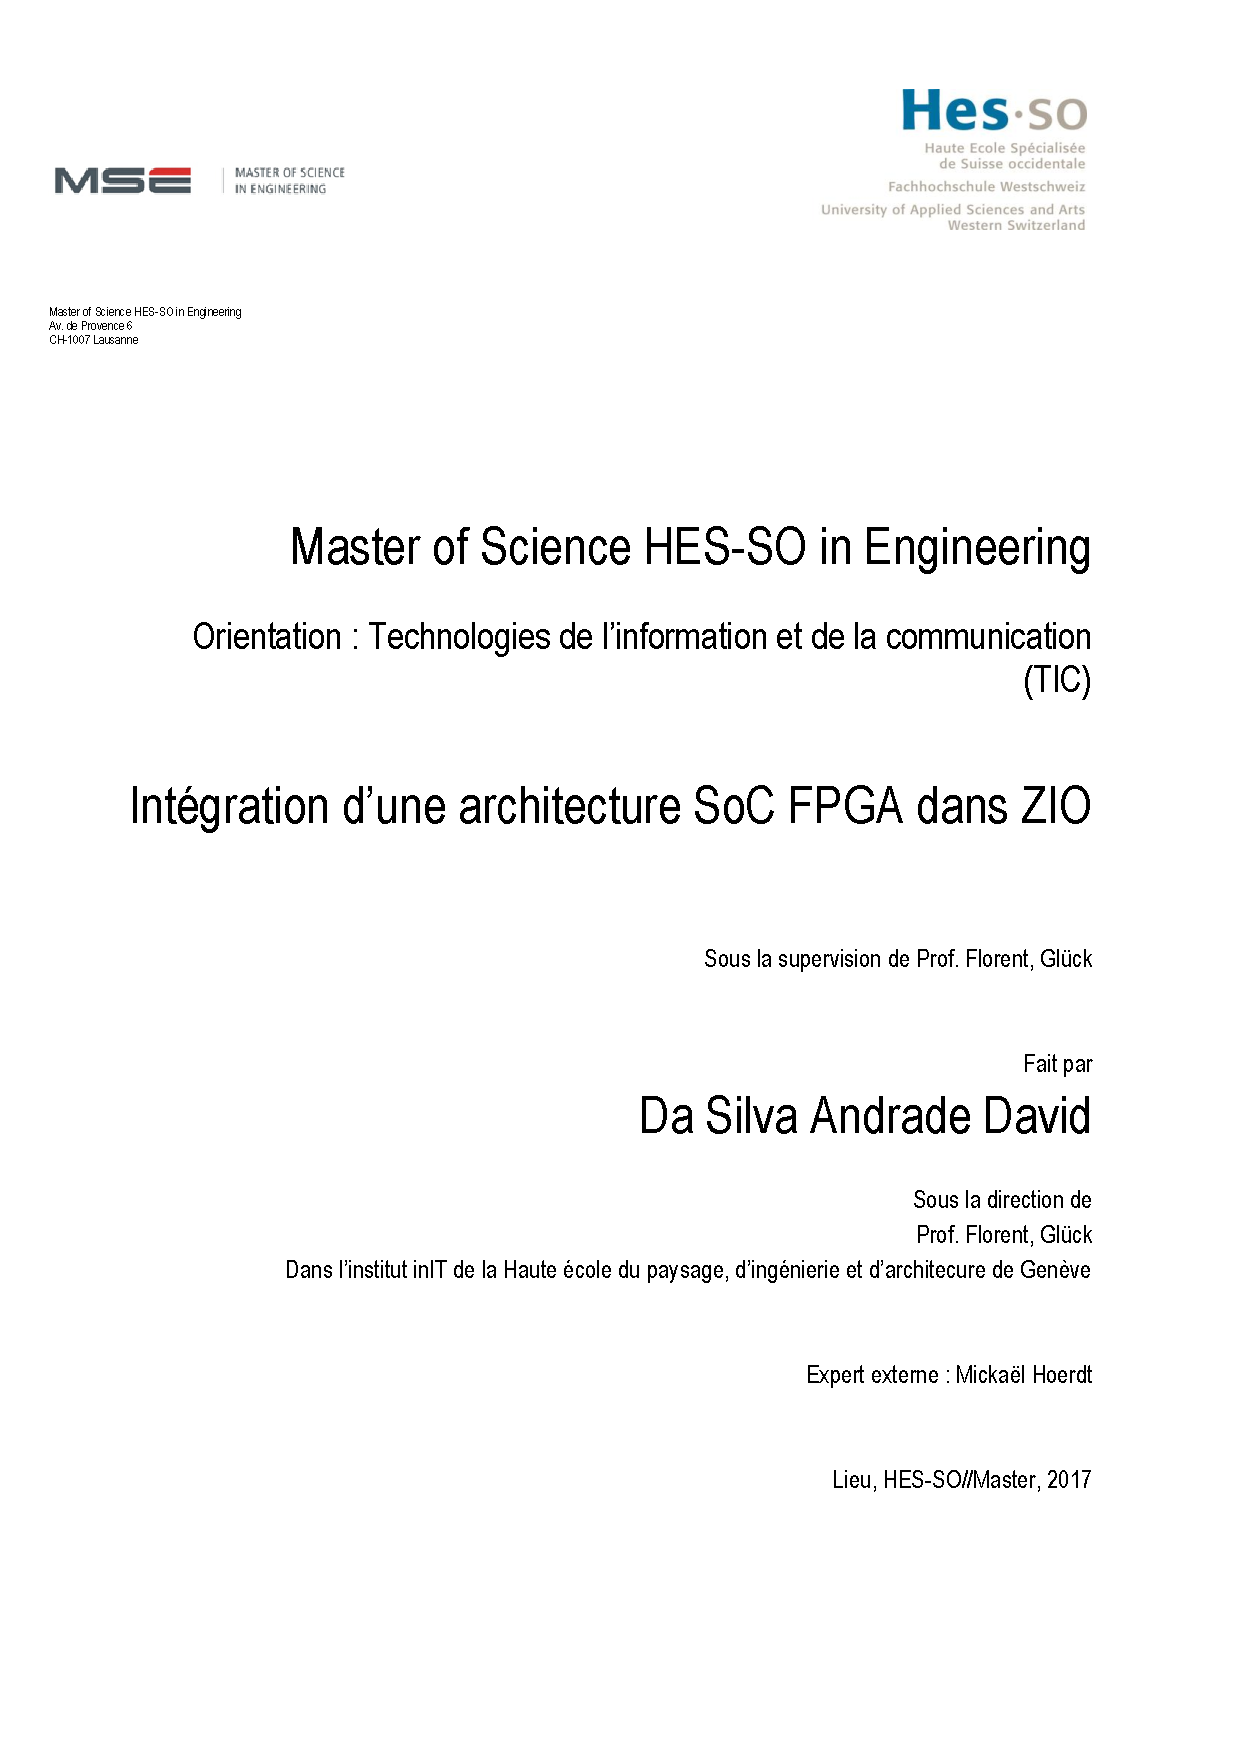
\includepdf{front_page.pdf}

% \begin{titlepage}
% \begin{center}

% \vspace*{.06\textheight}
% {\scshape\LARGE \univname\par}\vspace{1.5cm} % University name
% \textsc{\Large Projet d'approfondissement}\\[0.5cm] % Thesis type

% \HRule \\[0.4cm] % Horizontal line
% {\huge \bfseries \ttitle\par}\vspace{0.4cm} % Thesis title
% \HRule \\[1.5cm] % Horizontal line
 
% \begin{minipage}[t]{0.4\textwidth}
% \begin{flushleft} \large
% \emph{Author:}\\
% \authorname % Author name - remove the \href bracket to remove the link
% \end{flushleft}
% \end{minipage}
% \begin{minipage}[t]{0.4\textwidth}
% \begin{flushright} \large
% \emph{Supervisor:} \\
% \supname % Supervisor name - remove the \href bracket to remove the link  
% \end{flushright}
% \end{minipage}\\[3cm]
 
% \vfill

% \large \textit{A thesis submitted in fulfillment of the requirements\\ for the degree of \degreename}\\[0.3cm] % University requirement text
% \textit{in the}\\[0.4cm]
% \groupname\\\deptname\\[2cm] % Research group name and department name
 
% \vfill

% {\large \today}\\[4cm] % Date
% %\includegraphics{Logo} % University/department logo - uncomment to place it
 
% \vfill
% \end{center}


% \end{titlepage}

%----------------------------------------------------------------------------------------
%	DECLARATION PAGE
%----------------------------------------------------------------------------------------

% \begin{declaration}
% \addchaptertocentry{\authorshipname} % Add the declaration to the table of contents
% \noindent I, \authorname, declare that this thesis titled, \enquote{\ttitle} and the work presented in it are my own. I confirm that:

% \begin{itemize} 
% \item This work was done wholly or mainly while in candidature for a research degree at this University.
% \item Where any part of this thesis has previously been submitted for a degree or any other qualification at this University or any other institution, this has been clearly stated.
% \item Where I have consulted the published work of others, this is always clearly attributed.
% \item Where I have quoted from the work of others, the source is always given. With the exception of such quotations, this thesis is entirely my own work.
% \item I have acknowledged all main sources of help.
% \item Where the thesis is based on work done by myself jointly with others, I have made clear exactly what was done by others and what I have contributed myself.\\
% \end{itemize}
 
% \noindent Signed:\\
% \rule[0.5em]{25em}{0.5pt} % This prints a line for the signature
 
% \noindent Date:\\
% \rule[0.5em]{25em}{0.5pt} % This prints a line to write the date
% \end{declaration}

% \cleardoublepage

%----------------------------------------------------------------------------------------
%	QUOTATION PAGE
%----------------------------------------------------------------------------------------

% \vspace*{0.2\textheight}

% \noindent\enquote{\itshape Thanks to my solid academic training, today I can write hundreds of words on virtually any topic without possessing a shred of information, which is how I got a good job in journalism.}\bigbreak

% \hfill Dave Barry

%----------------------------------------------------------------------------------------
%	ABSTRACT PAGE
%----------------------------------------------------------------------------------------

\begin{abstract}
\addchaptertocentry{\abstractname} % Add the abstract to the table of contents
The Thesis Abstract is written here (and usually kept to just this page). The page is kept centered vertically so can expand into the blank space above the title too\ldots
\end{abstract}


%----------------------------------------------------------------------------------------
%	LIST OF CONTENTS/FIGURES/TABLES PAGES
%----------------------------------------------------------------------------------------

\tableofcontents % Prints the main table of contents

\listoffigures % Prints the list of figures

\listoftables % Prints the list of tables

%----------------------------------------------------------------------------------------
%	ACKNOWLEDGEMENTS
%----------------------------------------------------------------------------------------

\begin{acknowledgements}
\addchaptertocentry{Remerciements} % Add the acknowledgements to the table of contents
The acknowledgments and the people to thank go here, don't forget to include your project advisor\ldots
\end{acknowledgements}

%----------------------------------------------------------------------------------------
%	ABBREVIATIONS
%----------------------------------------------------------------------------------------

\begin{abbreviations}{ll} % Include a list of abbreviations (a table of two columns)

\textbf{DGSI} & \textbf{D}irection \textbf{G}énérale des \textbf{S}ystèmes d'\textbf{I}nformation \\
\textbf{POC} & \textbf{P}roof \textbf{O}f \textbf{C}oncept \\
\textbf{DASS} & \textbf{D}ata \textbf{A}ccess \textbf{S}ub-\textbf{S}ystem \\
\textbf{RNSS} & \textbf{R}adio \textbf{N}etwork \textbf{S}ub-\textbf{S}ystem \\

\textbf{UART} & \textbf{U}niversal \textbf{A}synchronous \\
\textbf{SPI} & \textbf{S}erial \textbf{P}eripheral \textbf{I}nterface \\
\textbf{I2C} & \textbf{I}nter-\textbf{I}ntegrated \textbf{C}ircuit \\
\textbf{LPWAN} & \textbf{L}ow-\textbf{P}ower \textbf{W}ide-\textbf{A}rea Network \\
\textbf{ABP} & \textbf{A}ctivation \textbf{B}y \textbf{P}ersonalization \\
\textbf{OTAA} & \textbf{O}ver-\textbf{T}he-\textbf{A}ir \textbf{A}ctivation \\


\end{abbreviations}

%----------------------------------------------------------------------------------------
%	PHYSICAL CONSTANTS/OTHER DEFINITIONS
%----------------------------------------------------------------------------------------

% \begin{constants}{lr@{${}={}$}l} % The list of physical constants is a three column table

% % The \SI{}{} command is provided by the siunitx package, see its documentation for instructions on how to use it

% Speed of Light & $c_{0}$ & \SI{2.99792458e8}{\meter\per\second} (exact)\\
% %Constant Name & $Symbol$ & $Constant Value$ with units\\

% \end{constants}

%----------------------------------------------------------------------------------------
%	SYMBOLS
%----------------------------------------------------------------------------------------

% \begin{symbols}{lll} % Include a list of Symbols (a three column table)

% $a$ & distance & \si{\meter} \\
% $P$ & power & \si{\watt} (\si{\joule\per\second}) \\
% %Symbol & Name & Unit \\

% \addlinespace % Gap to separate the Roman symbols from the Greek

% $\omega$ & angular frequency & \si{\radian} \\

% \end{symbols}

%----------------------------------------------------------------------------------------
%	DEDICATION
%----------------------------------------------------------------------------------------

%\dedicatory{For/Dedicated to/To my\ldots} 

%----------------------------------------------------------------------------------------
%	THESIS CONTENT - CHAPTERS
%----------------------------------------------------------------------------------------

\mainmatter % Begin numeric (1,2,3...) page numbering

\pagestyle{thesis} % Return the page headers back to the "thesis" style

% Include the chapters of the thesis as separate files from the Chapters folder
% Uncomment the lines as you write the chapters

\chapter*{Resumé}
\chapter{Introduction}
\label{1_introduction}


De nos jours, de plus en plus de villes proposent des données aux habitant. Ces données sont acquises en utilisant divers capteurs disséminés à travers la ville.

L'expression \textit{Smart City} est de plus en plus présente dans notre quotidien. C'est principalement dans une optique d'améliorer la qualité des services urbains ou de réduire leurs coûts que les institutions publiques sont intéressées par ce concept. 



Dans la canton de Genève, en Suisse, plusieurs données sont accessibles librement par la population. Ces données sont mises à disposition par le \textbf{Système d'Information du Territoire à Genève} (\textit{SITG}).




\section{Contexte}

Le canton de Genève a décidé proposer un projet de SmartCanton afin de laisser la possibilité à des entreprises ou des individuelles de proposer fournir des données afin d'alimenter une base de données communes. 

Afin de couvrir une plus grande zone possible, une technologie de type LPWAN (Low-Power Wide-Area Network) est utilisée. La technologie retenu pour ces capteurs a été le LoRa \cite{LPWANWik40:online}. LoRa est une modulation de fréquence (couche 1 du modèle OSI) propriétaire à l'entreprise Semtech. LoRa utilise différentes fréquences dans le monde en fonction des fréquences libres. En Europe il s'agit de la fréquence 868 MHz alors qu'en Amérique du Nord la fréquence de 915MHz est quand à elle utilisée. On dessus de cette couche physique on peut trouver différentes spécifications possibles. Celle utilisée dans ce projet est le LoRaWAN. LoRaWAN est la spécification proposée par la LoRa Alliance \cite{loraalli46:online}. 

Le projet SmartCanton doit également couvrir la sécurité, que ce soit au niveau du transfert des données, mais également sur l'authentification sur le réseau. Une fois un dispositif sur le réseau, les données échangées sont toujours chiffrées. Ceci est géré par la spécification LoRaWAN. 

La DGSI souhaite créer des clés d'authentification au réseau LoRa avec des temps de validité. Il y a donc la problématique d'échange de ces clés avec le périphérique quand l'une de ces clés arrive à péremption. A l'heure actuelle ces périphériques reçoivent toutes les clés lorsqu'ils sont programmés (en mode ABP) ou reçoivent des clés quand ils s'authentifient auprès d'un réseau (OTAA). 




\chapter{State of the art}
\label{2_state_of_the_art}


\section{\textit{Smart Cities}}



\section{LPWAN}



\section{\textit{Software}}

Pour l'implémentation logicielle plusieurs alternatives sont possibles. Dans le cas de l'utilisation de processeurs implémentant des communications sans fils, un \textbf{Real Time Operating System} (\textit{RTOS}) est nécessaire. 

\section{\textit{Hardware}}

Les dispositifs matériels sur le marché implémentant une interface de communication utilisent souvent deux processeurs. Un premier processeurs, souvent le moins puissant, est utilisé pour la gestion de l'interface de communication. Il s'occupe à lui seul de la communication avec l'extérieur. Ceci peut être une tâche coûteuse selon le type de protocole implémenté. Par exemple, si de la cryptographie rentre en jeu, une partie 

Celui-ci communique ensuite avec un processeur plus puissant via une interface de communication variant selon les implémentation. Ce deuxième processeur est à disposition de l'utilisateur pour toutes les tâches qu'il souhaite. Mais il doit souvent tenir compte que la communication avec le premier processeur coûte tout de même quelques ressources. A cause de ce type de structure mais aussi de la complexité à maintenir un système stable, un \textit{RTOS} doit être utilisé.\\


On trouve divers fabricants proposant des kits de développement orientés IoT et très facilement utilisable dans un concept SmartCity. L'un des plus connus est STMicroelectronics\footnote{\url{http://www.st.com/content/st_com/en.html}}. Il propose une très grande panoplie de capteurs pouvant êtres utilisés dans un grand nombre de situations\footnote{\url{http://www.st.com/en/evaluation-tools/stm32-nucleo-expansion-boards.html?querycriteria=productId=SC1971}}. Les kits de développement de STM sont souvent utilisés par des passionnés car ils sont très facile d'accès en terme de disponibilité mais aussi en terme de coût. On trouve ainsi des kits avec du WiFi, du NFS ainsi que du Bluetooth pour moins de 50 CHF. L'écosystème STM disposent d'une très grande communauté ainsi que de librairies très bien construisent qui offrent ainsi une aise lors de l'implémentation d'un projet personnel. Une grande partie de leurs kits de développement sont supportés par la plateforme mbed\footnote{\url{https://www.mbed.com/en/}} maintenue par la société de conception d'architecture de processeurs ARM. La plateforme mbed offre ainsi une suite de librairies facilitant également l'implémentation ainsi que la programmation. 

Un problème provenant de ces kit est la disponibilité. Certains de ces kits ne sont pas censé être utilisé pour des produits finaux. Ils restent des plateformes afin de pouvoir tester le produit vendu, ce qui n'oblige aucunement le vendeur a garantir une disponibilité ni même une compatibilité entre les différents designs. Certaines cartes de développement peuvent arrêter d'être produite du jour du lendemain. C'est un problème conséquent si cette carte est utilisée dans un produit commercial. 

Il restent au final des kits de développement, qui sont bon marché. Ils permettent de créer très facilement des prototypes très rapidement. Ils sont donc idéaux pour des \textit{proof of concept}. Mais lorsque l'utilisateur désire avoir un produit final, il est forcé à implémenter le processeur directement dans une carte électronique sur mesures.

On voit ainsi plusieurs acteurs sur le marché proposant des kits. Les plus grand fabricants de microcontrôleurs sont STM, NXP ou Texas Instruments, proposant chacun des plateformes et des exemples afin de tester leurs produits. \\


Libelium\footnote{\url{http://www.libelium.com/}} est également un acteur dans le marché des SmartCities. Une différence avec STMicroelectronics est déjà que Libelium n'est pas un fabricant de microcontrôleur en tant que tel. Ils proposent plusieurs cartes, mais la plupart basées sur un processeur d'Atmel ATMEGA1281 
Cela rend l'utilisation de leurs équipement très simple. Mais malheureusement limite la puissance de calcul car ce processeur n'est pas très puissant et l'utilisation de l'environnement Arduino pour la programmation réduit grandement la flexibilité et la puissance de calcul pour l'utilisateur.



\section{Communication sans fil à 2.4 GHz}
\label{sec_2_4_GHz}

La plage de fréquence autour de 2.4 GHz est l'une des plus utilisée au monde. Ceci est dû au fait que celle-ci peut être utilisée sans avoir besoin d'une licence provenant d'une autorité de certification et cela dans tous les pays du monde \cite{ISMbandW77:online}. Plusieurs autres fréquences sont également ouvertes dans le monde, mais le succès de cette plage provient de trois facteurs : 
\begin{itemize}
    \item La taille de l'antenne. En effet, un principe simple en radio communication est que plus la fréquence est élevée et plus l'antenne peut être compacte. On peut facilement le constater avec la \autoref{eq:dipole_base_formula} représentant la longueur d'un dipôle \cite{DipoleLe18:online}. La constante A dépend principalement la longueur de l'antenne en fonction de l'épaisseur du matériaux utilisé. Cette constante se situe typiquement entre 0.96 et 0.98 \cite{DipoleLe18:online}. Il est possible de trouver divers graphique permettant d'obtenir la valeur de cette constante \footnote{\url{http://www.radio-electronics.com/info/antennas/dipole/length-calculation-formula.php}}, facilitant ainsi son dimensionnement.
    
    
    \begin{equation}
    \label{eq:dipole_base_formula}
    Length \ dip\hat{o}le [m] = \frac{150 * A}{freq [MHz]}
    \end{equation}

    \begin{equation}
    \label{eq:dipole_2_4GHz}
    Longeur \ dip\hat{o}le [m] = \frac{150 * 0.98}{2400} = 0.06125 = 6.125 [cm]
    \end{equation}
    
    \begin{equation}
    \label{eq:dipole_433MHz}
    Longeur \ dip\hat{o}le [m] = \frac{150 * 0.98}{433} \approx 0.33949 = 33.949 [cm]
    \end{equation}
    
    En utilisant l'\autoref{eq:dipole_base_formula} avec 2.4 GHz (\autoref{eq:dipole_2_4GHz}) et 433 MHz (\autoref{eq:dipole_433MHz}) on observe bien l'influence de la fréquence sur ce dipôle et donc la place qui devra être allouée à une antenne sur une carte électronique. Grâce à une miniaturisation qui devient donc raisonnable on peut ainsi facilement offrir des périphériques compactes.
    
    \item La technologie électronique disponible pour gérer ces hautes fréquences. Grâce à l'avancée dans les domaines de l'électronique et de la microélectronique, il est maintenant possible d'avoir des circuit intégrés pouvant offrir la modulation à cette fréquence et cela en ayant un taille raisonnable. Le microcontrôleur utilisé dans ce projet offre par exemple un \textit{package} de 3.9mmx3.8mm et ne nécessitant aucun élément électronique externe pour l'antenne. Ceci permet de créer une carte électronique extrêmement compacte. Le prix de ce type de technologie est de plus en plus négligeable lors du développement(cf. \autoref{subsect:microcontroleur} pour un comparatif plus approfondi des microcontrôleur compatible Bluetooth avec des indications de prix).
    
    \item La distance couverte par cette plage de fréquence. Cette fréquence permet d'avoir une distance tout à fait raisonnable entre la deux périphériques. Le Bluetooth 5.0 peut ainsi atteindre, en théorie, jusqu'à 240m dans un environnement ouvert. 


    
\end{itemize}

La fréquence de 2.4GHz est utilisée par de nombreux protocoles. On y trouve le Bluetooth, le Wi-Fi, 
ou une panoplie d'autres standards, comme le IEEE 802.15.2. Si on prend l'exemple d'un smartphone ou d'une tablette. Les seuls protocoles supportés universellement sur toutes ces plateformes sont le Bluetooth ainsi que le Wi-Fi. Le problème de ce dernier est l'impacte sur la consommation des appareils, mais avec comme avantage d'avoir une grand débit. Le Bluetooth est lui plutôt utilisé lors de la communication avec des périphériques proches de l'utilisateur et ne nécessitant pas un aussi grand débit de données, offrant ainsi une plus grande autonomie. Le Wi-Fi est lui plus utilisé dans le cadre d'un besoin de communication avec des données externes, provenant par exemple d'Internet.\\

Même la modulation LoRa est maintenant disponible dans cette fréquence grâce au circuit intégré Semtech SX1280\footnote{\url{http://www.semtech.com/wireless-rf/rf-transceivers/sx1280/}}. \\

Le marché du Bluetooth est en pleine expansion depuis plusieurs années. Cette tendance provient surtout dû au faite de la démocratisation des smartphones. Le Bluetooth est en effet l'une des rares interfaces de communication présente sur tous les dispositifs comme pour les communication LTE ou WiFi. L'évolution dans ce domaine est 


Le Bluetooth 5.0 a été officiellement annoncé le 16 juin 2016. Néanmoins, les premiers microcontrôleur implémentant toutes les fonctionnalités de ce protocole n'ont été annoncé que pour courant 2017. Une partie des prérequis pour passer au Bluetooth 5.0 ne nécessitent qu'une mise à jour logicielle. Par exemple, l'augmentation de la taille des \textit{advertissements}, qui passent de maximum 31 bytes à 255 bytes. Il aurait été intéressant d'avoir un processeur compatible Bluetooth 5.0. Mais peu sont actuellement disponibles, même si de 



\section{LoRa}

Le cas du LoRa est plus problématique que celui du Bluetooth. En effet, un seul fabricant est à l'heure actuelle autorisé à produire les puces avec la modulation LoRa, il s'agit de la société Semtech\footnote{\url{http://www.semtech.com/}}. 

Cela réduit donc considérablement le nombre de possibilités. Semtech a annoncée une collaboration avec STMicroelectronics pour développeur un processeurs dans lequel on retrouve un STM32 avec en interne un coeur attribué uniquement à la modulation LoRa et l'implémentation du protocole LoRaWAN.


Mais en attendant ce microcontrôleur est en cours de développeur. Murata, un célèbre fabricant de semiconducteur s'est donc allié avec STMicroelectronics afin d'offrir un module nommé CMWX1ZZABZ-078. Ce module est composé en interne d'un STM32L0 basé sur une architecture ARM Cortex M0+ qui communique en interne avec un SX1276 de Semtech pour la communication LoRa.

Ce module permet surtout une économie de place sur la carte électronique. Sa taille est de 12.5x11.6x1.76mm permettant ainsi facilement son placement sur une carte électronique. Il permet également de réduire les temps d'implémentation car une suite de librairie est disponible 




\section{SmartCanton}



Le canton Genève s'est donné comme objectif stratégique de devenir un pilier dans le domaine des smart cities d'ici 2030 \cite{Genevebr38:online}. Celui-ci deviendrai ainsi un Smart Canton dans lequels les utilisateurs pourraient accéder aux données capturées et les utiliser dans le cadre de projets personnels mais également commerciaux. Le but, une fois les données capturées est de les faire parler. Pour cela on peut imaginer plusieurs algorithmes de Machine Learning permettant de créer des modèles afin de pouvoir mieux conseiller les habitants, analyser les risques et également réduire les coûts de certaines actions qui nécessecitent actuellement la présence d'une personne physique à proximité. 

Un POC (\textit{\textbf{P}roof \textbf{O}f \textbf{C}oncept}) a donc été lancé dans ce sens afin de pouvoir présenter différentes approchent de ce SmartCanton ainsi que les limitations et les opportunités des différentes technologies possibles. La technologie retenue pour pouvoir remonter les données a été le LoRa. 



\chapter{Hardware}
\label{3_hardware}

Ce chapitre présente toute l'implémentation de la carte électronique qui a été réalisée dans ce projet. On y présente celle-ci avec la description des composants. Le choix de ces composants y est également évoqué.


\section{Introduction}

Après avoir analyser les différents besoin 



\section{Architecture}

Nous désirions utiliser deux processeurs sur la carte électronique. Nous avions donc deux implémentations possibles. Les \autoref{fig:hardware_option1} et \autoref{fig:hardware_option2} illustrent toutes deux ces deux options. La première consiste à utilise un processeur LoRa comme processeur principal du système. C'est à dire un processeur sur lequel la communication LoRa est gérée en plus de la gestion des différents périphériques de la carte. Comme par exemple le GPS, un accéléromètre, etc. Le processeur gérant le Bluetooth serait donc comme un simple périphérique pour le processeur LoRa. Une API doit être mise en place pour faciliter l'échange d'information entre les deux. La deuxième possibilité est d'inverser les rôle des processeurs. Le processeur principal serait celui qui gère les protocoles en 2.4 GHz et communiquant périodiquement avec le processeur LoRa afin d'envoyer et recevoir des données provenant du réseau.

\begin{figure}[ht!]
    \centering
    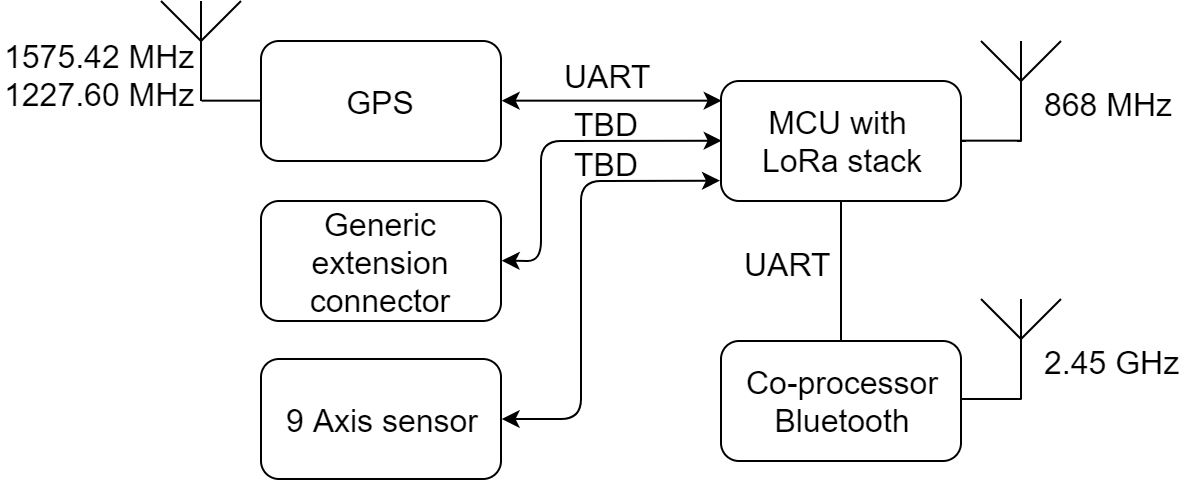
\includegraphics[width=\textwidth]{Figures/hardware/master_onepage_option1.png}
    \caption{Architecture option numéro 1}
    \label{fig:hardware_option1}
\end{figure}

\begin{figure}[ht!]
    \centering
    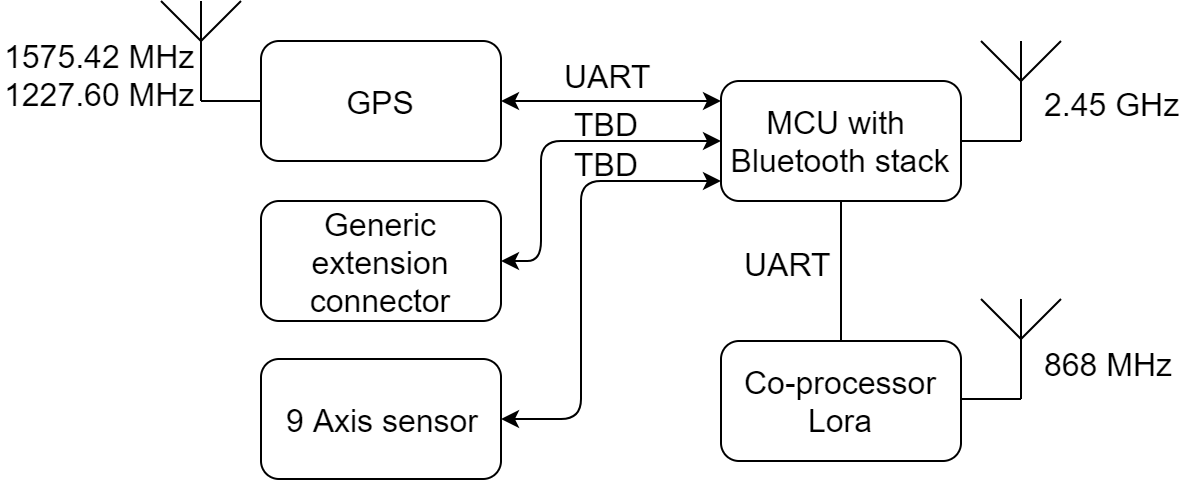
\includegraphics[width=\textwidth]{Figures/hardware/master_onepage_option2.png}
    \caption{Architecture option numéro 2}
    \label{fig:hardware_option2}
\end{figure}

L'architecture choisie est la numéro 2. Nous avons donc tous les périphériques qui sont connectés au processeur s'occupant du Bluetooth. Le processeur avec l'interface LoRa, lui ne s'occupe que de communiquer les évènements de réception de données ainsi que de transférer les messages provenant depuis le processeur 2.4 GHz.

Il est également plus simple de faire une API pour le LoRa, le nombre de données et paramètres configurables sont moins importants que dans le cas des communications 2.4GHz. Si on souhaite donc faire une API entre les deux processeur, il est nécessaire de tenir compte de la complexité de ceux-ci. Les accès LoRa sont également plus ponctuelles. Le nombre de paquets envoyé par heures sont très faibles à comparer à ce qui est réalisable en 2.4 GHz. On peut ainsi faire en sorte que le processeur soit en mode très basse consommation en attendant une commande de la part du processeur principal ou la réception d'un paquet LoRa sur son antenne.


\section{Choix du matériel}

Cette section a pour rôle d'expliquer les différents choix effectués pour les composants présents sur la DevBox. 

\subsection{Microcontrôleur}
\label{subsect:microcontroleur}

Pour choisir quel microcontrôleur était l'idéal pour le cahier des charges un comparatif approfondis a été effectué. Ce comparatif est visible sur le \autoref{mcu_table}. Donc premièrement, un des point qui a été retenu a été le type de protocole qui est supporté par le processeur. Le Bluetooth Low Energy étant un prérequis, cela nous a permis de faire en sorte d'avoir un premier filtre. C'est pour cela que tous les microcontrôleur affichés disposent tous cette fonctionnalité. Néanmoins, dans le Bluetooth Low Energy on y trouve la norme 4.2 qui a été annoncée le 2 décembre 2014 \cite{Bluetoot59:online} et la norme 5.0 annoncée elle le 16 juin 2016. Cette dernière n'était malheureusement pas encore parfaitement supportée par tous les fabricants de microcontrôleur. Comme expliqué précédemment sous la \autoref{sec_2_4_GHz}, une simple mise à jour logicielle permet de passer un microcontrôleur en Bluetooth 5.0, du moins, en garantissant les fonctionnalité primordiales du protocole. Les microcontrôleur affichés dans le tableau disposait, à la date du 1 octobre 2017, que des fonctionnalités listées.

Après le Bluetooth, le deuxième type de protocole est le IEEE 802.15.4 \cite{IEEE802137:online}. Ce standard IEEE n'est pas un protocol en tant que tel, mais c'est un modèle qui est respecté par plusieurs ptotocoles du commerce. On trouve différents protocoles qui sont utilisable avec ce standard, comme le ZigBee, WirelessHART, MiWi, SNAP, ou encore Thread. Ce standard est de plus en plus utilisé pour la domotique. Il permet de facilement créer des réseaux maillés permettant ainsi une grande couverture de l'habitation.

Un dernier moyen de communication en dessous d'un GHz. Si le processeur supporte cela, ça peut être un avantage. Néanmoins, la communication dans cette plage de fréquence a quelques désavantages, en commençant par la taille de l'antenne qu'il faut utiliser. La consommation du processeur est également affectée, pouvant atteindre jusqu'à 100 mA (cf. EFR32M datasheet).

LoRa rentre dans cette catégorie, mais uniquement les processeurs fournis par Semtech peuvent implémenter la modulation. Ils ne sont à l'heure actuelle pas assez évolués pour pouvoir être utilisé comme unique processeur gérant à la fois du 2.4 GHz avec en parallèle une interface LoRa (868 ou 433 MHz).

On a ensuite l'aspect consommation qui rentre en jeu. Afin d'être le plus proche possible en terme de comparaison, la consommation en émission à été retenu pour la fréquence de 2.4 GHz avec une puissance de 0 dBm en sortie. Plus cette consommation est faible et plus notre système aura la possibilité d'être autonome grâce à sa batterie. 

Finalement, les deux derniers points à retenir sont la taille des mémoires (RAM et Flash), qui selon leur taille nous permettront de faire un programme plus complexe et le coût à l'unité du microcontrôleur. Les prix ont été sélectionné pour une seule unité sur le site d'achat Mouser\footnote{\url{http://www.mouser.ch/}} Suisse. 

Après

Le microcontrôleur retenu a donc été le KW41Z de NXP. Celui-ci a été initialement développer par l'entreprise Freescale qui depuis le lancement de ce produit a été rachetée par NXP. 


\begin{sidewaystable}[!ht]
\centering
\caption{Table}
\label{tab:mcu_table}
\begin{tabular}{|l|l|l|c|c|c|c|l|l|c|c|l|}
\hline
\multicolumn{1}{|c|}{\textbf{Manufacturer}} & \multicolumn{1}{c|}{\textbf{Model}} & \multicolumn{1}{c|}{\textbf{CPU}} & \textbf{\begin{tabular}[c]{@{}c@{}}BLE\\ 4.2\end{tabular}} & \textbf{\begin{tabular}[c]{@{}c@{}}BLE\\ 5.0\end{tabular}} & \textbf{\begin{tabular}[c]{@{}c@{}}IEEE\\     802.15.4\end{tabular}} & \textbf{\begin{tabular}[c]{@{}c@{}}Sub\\     1GHz\end{tabular}} & \multicolumn{1}{c|}{\textbf{\begin{tabular}[c]{@{}c@{}}Receive \\     Current\end{tabular}}} & \multicolumn{1}{c|}{\textbf{\begin{tabular}[c]{@{}c@{}}Transmit\\ Current \\ (@ 2.4Ghz, \\ @ 0dBm)\end{tabular}}} & \textbf{\begin{tabular}[c]{@{}c@{}}Flash/\\     SRAM\end{tabular}} & \textbf{Disponibility} & \multicolumn{1}{c|}{\textbf{Price}} \\ \hline
NXP & KW41Z & \begin{tabular}[c]{@{}l@{}}Cortex\\ M0+\end{tabular} & Yes & No & Yes & No & 6.8 mA & 6.1 mA & \begin{tabular}[c]{@{}c@{}}512 kB\\ / 128 kB\end{tabular} & Yes & 6.34 CHF \\ \hline
NXP & QN908x & \begin{tabular}[c]{@{}l@{}}Cortex\\ M4F\end{tabular} & Yes & Yes & No & No & 3.4 mA & 3.4 mA & \begin{tabular}[c]{@{}c@{}}512 kB\\ / 128 kB\end{tabular} & Yes & 5.87 CHF \\ \hline
\begin{tabular}[c]{@{}l@{}}Texas\\     Instrument\end{tabular} & CC2650 & \begin{tabular}[c]{@{}l@{}}Cortex\\ M3\end{tabular} & Yes & No & Yes & No & 6.2 mA & 6.8 mA & \begin{tabular}[c]{@{}c@{}}128 kB\\ / 128 kB\end{tabular} & Yes & 6.34 CHF \\ \hline
\begin{tabular}[c]{@{}l@{}}Texas\\     Instrument\end{tabular} & CC2640R2F & \begin{tabular}[c]{@{}l@{}}Cortex\\ M3\end{tabular} & Yes & Yes & No & No & 6.1 mA & 7.0 mA & \begin{tabular}[c]{@{}c@{}}128 kB\\ / 20 kB\end{tabular} & Yes & 6.34 CHF \\ \hline
\begin{tabular}[c]{@{}l@{}}Nordic \\     Semiconductor\end{tabular} & NRF52832 & \begin{tabular}[c]{@{}l@{}}Cortex\\ M4F\end{tabular} & Yes & Yes & No & No & 5.4 mA & 5.3 mA & \begin{tabular}[c]{@{}c@{}}512 kB\\ / 64 kB\end{tabular} & Yes & 5.51 CHF \\ \hline
\begin{tabular}[c]{@{}l@{}}Nordic \\     Semiconductor\end{tabular} & NRF52840 & \begin{tabular}[c]{@{}l@{}}Cortex\\ M4F\end{tabular} & Yes & Yes & Yes & No & N/A & N/A & \begin{tabular}[c]{@{}c@{}}1MB /\\     256 kB\end{tabular} & No & N/A \\ \hline
Silicon Labs & \begin{tabular}[c]{@{}l@{}}EFR32M\\ G12P433\\ F1024GL125\end{tabular} & \begin{tabular}[c]{@{}l@{}}Cortex\\ M4F\end{tabular} & Yes & Yes & Yes & Yes & 9.3 mA & 9.5 mA & \begin{tabular}[c]{@{}c@{}}1MB /\\     256 kB\end{tabular} & Yes & 13.5 CHF \\ \hline
\end{tabular}
\end{sidewaystable}



\subsection{Alimentation et batterie}

Le système doit pouvoir être autonome, afin de garantir cela, une batterie peut être ajoutée. La capacité de cette batterie reste au choix de l'utilisateur. 

L'utilisateur peut recharger la batterie à l'aide du connecteur micro-USB présent sur la carte. 


L'aspect autonomie peut être encore plus poussé en connectant un panneau solaire directement sur la carte. Celui-ci a son propre connecteur dédié en entrée. Ce panneau permet ainsi de directement charger la batterie qui fournira à son tour la tension pour le système. 

Pour gérer la tension élevée du panneau solaire un circuit intégré nommé BQ24210\footnote{\url{http://www.ti.com/product/BQ24210}} est utilisé. Ce dernier s'occupe directement de la recharge de la batterie supportant en entrée jusqu'à 20V de tension. Il est capable de fournir jusqu'à 800 mA à la batterie, tout en protégeant celle-ci en cas de surtension. Il accepte également la possibilité de recharger avec une tension de 5V, permettant ainsi la recharge directement depuis une prise USB. 


Une batterie est donc couplée au système. Celle-ci n'a pas de restriction de taille, elle doit simplement être de type Li-Ion à cause de la tension et de la courbe de charge fournie par le BQ24210. La batterie n'a pas besoin d'offrir un circuit de protection contre les surcharges ni les décharges profondes. Comme expliqué précédemment, le BQ24210 arrête la charge lorsque la batterie est pleine et afin de protéger la batterie des décharges profondes 

L'ensemble de la carte est alimentée en 3.3V à l'aide d'un régulateur TPS62291. Celui-ci peut fournir un courant maximum de 1A. Ce haut courant a juste été pris comme précaution selon le type de cartes d'extensions que l'utilisateur souhaite ajouter à la DevBox. Il dispose d'un courant typique de fonctionnement très faible de 15 uA, pouvant ainsi consommer un minimum si on souhaite mettre toute la carte en basse consommation.

\subsection{Coprocesseur LoRa}

La communication via LoRa est uniquement possible en utilisant les circuits proposé par l'entreprise Semtech. Semtech propose une gamme de circuit qui est visible à l'adresse suivante : 
\begin{center}
    \url{{http://www.semtech.com/wireless-rf/lora.html}}
\end{center}

Néanmoins, tous les circuit intégrés proposer sur le site de Semtech sont des périphériques qu'il faut ensuite relier avec un microcontrôleur via une communication SPI. Afin de palier à cela, plusieurs fabricants ont développés des chips intégrant un processeur couplé à un module de Semtech. Cela permet ainsi 


\subsection{Périphériques}
\subsubsection{LEDs}

Chaque microcontrôleur a à sa disposition 4 LEDs. Une bleu, une verte, une rouge ainsi qu'une jaune. Ces LEDs sont contrôlables via des GPIOs avec un état bas pour les allumés. 

\subsubsection{Buttons}

Chaque microcontrôleur a à sa disposition 2 boutons poussoirs. Ceux-ci produisent un état bas sur les GPIOs lorsque le bouton est préssé.


\subsubsection{Plateforme inertielle 9 axes}

La DevBox dispose d'une plateforme inertielle 9 axes (accéléromètre, gyroscope et magnétomètre) intégrés dans un même circuit électronique. Il s'agit d'un BNO055 du fabricant Bosch Sensortec dont la communication s'effectue via un bus I2C relié au processeur principal (KW41Z). L'adresse I2C est configurable en foncton de l'état de la pin COM3 du module. Deux résistances (R11 et R13, une seule doit être placée) permettent de choisir le dernier bit de l'adresse. Si la résistance R11 est placée, le périphérique a alors l'adresse 0x29. Si c'est la résistance R13, cette adresse est 0x28.

Le BNO055 a été crée avec la problématique de la consommation en tête. Dans son mode le plus bas, nommé \textit{Suspend Mode}, il ne consomme que 40 uA. 


\subsubsection{Qualité de l'air ambiant}

Une capteur de qualité de l'air a également été intégré sur la DevBox. Il s'agit du BME680 de Bosch Sensortec. Celui-ci ne mesure pas seulement la qualité de l'air, il mesure également la pression ambiante, la température, l'humidité et le gaz. Pour la mesure du gaz il s'agit des Volatile Organic Compounds\footnote{\url{}} (VOC), avec lesquels ont obtient une qualité globale de l'air ambiant.


\subsubsection{GPS}

La DevBox peut également être équipée d'un GPS si besoin. Celui-ci étant assez coûteux, il ne sera pas forcément monté sur toutes les cartes. Le GPS peut être utilisé si on souhaite tracker un objet en déplacement avec une très grande précision.
Il peut également être utilisé pour corréler la localisation obtenue via LoRa avec une position réeelle. En effet, comme expliqué 


\chapter{Sécurité}






\section{IEEE 802.15.4 et les protocoles dérivés}

Étant donné que le microcontrôleur choisi supporte le standard IEEE 802.15.4, il est intéressant de faire une petit analyse sur la sécurité implémentée dans ce standard. 

Le standard IEEE 802.15.4 décrit des procédures de sécurité. Le standard décrit quel algorithme de cryptage doit être utilisé pour chiffrer les données à transmettre \cite{Security81:online}. Cependant, le standard ne spécifie pas comment les clés doivent être échangées ni l'authentification de celles-ci. Le standard laisse cela aux couches supérieures. 


Le protocole ZigBee, qui est le protocole le plus répendu basé sur le standard IEEE 802.15.2.


% IEEE 802.15.4 sets the encryption algorithm to use when cyphering the data to transmit, however,  the standard does not specify how the keys have to be managed or what kind of authentication policies have to be applied. These issues are treated in the upper layers which are managed by technologies such as ZigBee.


\section{Bluetooth}




\section{LoRa}
\label{sec_lora_security}





\chapter{Gestion du projet}
\section{Planning}

\subsection{}


%----------------------------------------------------------------------------------------
%	THESIS CONTENT - APPENDICES
%----------------------------------------------------------------------------------------

\appendix % Cue to tell LaTeX that the following "chapters" are Appendices

% Include the appendices of the thesis as separate files from the Appendices folder
% Uncomment the lines as you write the Appendices

% Appendix Template

\chapter{counter.vhd} % Main appendix title

\label{AppendixCounterVHDL} % Change X to a consecutive letter; for referencing this appendix elsewhere, use \ref{AppendixX}

\lstinputlisting[language=VHDL]{Appendices/counter.vhd}

%----------------------------------------------------------------------------------------
%	BIBLIOGRAPHY
%----------------------------------------------------------------------------------------

\printbibliography[heading=bibintoc]

%----------------------------------------------------------------------------------------

\end{document}  
